% Welcome, Math for Math's sake folks!
%
% My idea is to use this file way to share solutions, questions, and comments.
%
% Feel free to edit any part of it, and add ``Your name:your comment, question, or solution'' so we know who is asking what.
%
% You don't have to worry too much about making mistakes in LaTeX format: ShareLatex keeps track of the file's history, so it's pretty easy to fix mistakes.  There's help here if you want to learn LaTeX and ShareLatex: https://www.sharelatex.com/learn
%
% If you're a techy person, this is also linked to a github repo here: https://github.com/mkoconnor/Math-for-Math-s-Sake-Logic-chapters-5-6-7-and-maybe-8 Feel free to submit a pull request.  If you've never heard of github, just ignore this paragraph.
%
% This is a total experiment, and I'm not sure if will people will like or use it, but let's find out!
\documentclass{article}
\usepackage[utf8]{inputenc}
\usepackage{tikz}
\usetikzlibrary{arrows,automata,positioning}

\title{Logic, chapters 5, 6, 7, and (maybe!) 8}
\author{Math for Math's Sake}
\newcommand\s{\section*}
\renewcommand\ss{\subsection*}
\newcommand\sss{\subsubsection*}
\newcommand\ms{Michael's solution: } % easy way to mark my solutions
\newcommand\pf{Peter's solution: } % Same for mine
\begin{document}
\maketitle
\s{5 Abacus Machines}
\ss{5.1}
\ms Suppose $x$ is stored in register $n$ and $y$ in register $m$.  The following abacus machine will put the output in register $n$.

\begin{center}
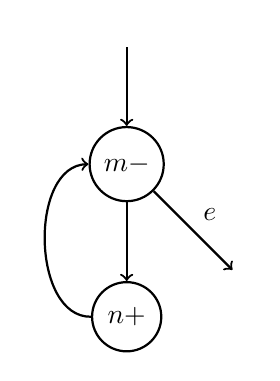
\begin{tikzpicture}[auto]
\tikzstyle{every path}=[thick];
\node (start) {};
\node[state] (subm) [below=of start] {$m{-}$};
\node (end) [below right=of subm] {};
\node[state] (addn) [below=of subm] {$n{+}$};
\path[->] (start) edge (subm);
\path[->] (subm) edge (addn);
\path[->] (subm) edge node {$e$} (end);
\path[->] (addn) edge [bend left=90] (subm);
\end{tikzpicture}
\end{center}

\ss{5.2}
\ms Suppose $x$ is stored in register $n$.  The following abacus
machine will put $\mathrm{sg}(x)$ in register $m$, assumed empty to begin with.

\begin{center}
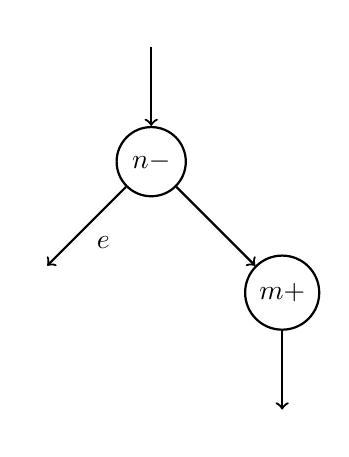
\begin{tikzpicture}[auto]
\tikzstyle{every path}=[thick];
\node (start) {};
\node[state] (subn) [below=of start] {$n{-}$};
\node[state] (addm) [below right=of subn] {$m{+}$};
\node (end1) [below=of addm] {};
\node (end2) [below left=of subn] {};
\path[->] (start) edge (subn);
\path[->] (subn) edge (addm);
\path[->] (addm) edge (end1);
\path[->] (subn) edge node {$e$} (end2);
\end{tikzpicture}
\end{center}
\ss{5.3}
\ms Since we know that exponentiation and subtraction are abacus computable, we know that $f(x)=1-0^x$ is abacus computable.  But this is equal to
$\mathrm{sg}(x)$, since $1-0^0 = 0$ but $1-0^x = 1$ for $x>0$.
\ss{5.4}
\ss{5.5}
\ss{5.6}
\ss{5.7}
\ss{5.8}
\ss{5.9}
\ss{5.10}
\pf First, create the equivalent Turing machine using the methods in section 5.2, then number them using the method on p. 36.
\ss{5.11}
\ms This is a standard argument: let $d$ be the function as described in the problem, and let $\lceil d\rceil$ be the natural number in the given encoding.  Then either $d(\lceil d\rceil) = 0$ or $d(\lceil d\rceil) = 1$.  Both cases are impossible by the definition of $d$.

\s{6 Recursive Functions}
% Some helper commands for the functionals defined in the text
\newcommand\id{\mathrm{id}} % identity
\newcommand\Cn{\mathrm{Cn}} % composition
\renewcommand\Pr{\mathrm{Pr}} % primitive recursion
\newcommand\Mn{\mathrm{Mn}} % minimization

\ss{6.1}
Suppose $f(x,y)$ is recursive.
\sss{6.1(a)}
\ms Then $g(x,y) = f(y,x)$ is recursive by $g(x,y) = \Cn[f,\id^2_2,\id^2_1]$
\sss{6.1(b)}
\ms And $h(x) = f(x,x)$ is recursive by $h(x) = \Cn[f,\id^1_1,\id^1_1]$
\sss{6.1(c)}
\ss{6.2}
\ss{6.3}
\ss{6.4}
\ss{6.5}
\ss{6.6}
\ss{6.7}
\ss{6.8}
\ss{6.9}

\s{7 Recursive Sets and Relations}
\ss{7.1}
\ss{7.2}
\ms We know that the relation $y^z\leq x$ is primitive recursive, since we know that exponentiation is primitive recursive from the 
last chapter.  $\mathrm{lg}(x, y)$ is the maximum $z$ for which
this is true.  In general, maximization isn't a primitive recursive or even a recursive operation, however we can put a bound on $z$: it can be no bigger than $x$, for example.  Thus we can use bounded maximization, which by Corollary 7.6, gives a primitive recursive function.
\ss{7.3}
\ss{7.5}
\ss{7.12}
\ss{7.13}
\ss{7.14}
\ss{7.15}
\ss{7.16}
\ss{7.17}

\s{8 Equivalent Definitions of Computability}
\ss{8.1}
\ss{8.2}
\end{document}
